\scanpage{27}

% upper left L1–6
\diagram{\begin{tikzcd}[ampersand replacement=\&,execute at end picture={\begin{scope}[x=.75cm,y=.75cm]\coordinate (g000) at (0,4);
\coordinate (g001) at (0.8,4);
\coordinate (g002) at (1.6,4);
\coordinate (g010) at (0,3.24);
\coordinate (g011) at (0.8,3.24);
\coordinate (g012) at (1.6,3.24);
\coordinate (g020) at (0,2.48);
\coordinate (g021) at (0.8,2.48);
\coordinate (g022) at (1.6,2.48);
\coordinate (g100) at (5,4);
\coordinate (g101) at (5.8,4);
\coordinate (g102) at (6.6,4);
\coordinate (g110) at (5,3.24);
\coordinate (g111) at (5.8,3.24);
\coordinate (g112) at (6.6,3.24);
\coordinate (g120) at (5,2.48);
\coordinate (g121) at (5.8,2.48);
\coordinate (g122) at (6.6,2.48);
\coordinate (g200) at (2,-0.4);
\coordinate (g201) at (2.8,-0.4);
\coordinate (g202) at (3.6,-0.4);
\coordinate (g210) at (2,-1.1600000000000001);
\coordinate (g211) at (2.8,-1.1600000000000001);
\coordinate (g212) at (3.6,-1.1600000000000001);
\coordinate (g220) at (2,-1.92);
\coordinate (g221) at (2.8,-1.92);
\coordinate (g222) at (3.6,-1.92);

\node[anchor=center,inner sep=1.2pt] at (g000) {$\unsure{\zeta|\xi}_{1}$};
\node[anchor=center,inner sep=1.2pt] at (g001) {$\zeta_{2}$};
\node[anchor=center,inner sep=1.2pt] at (g002) {$\zeta_{3}$};
\node[anchor=center,inner sep=1.2pt] at (g010) {$\zeta_{1}'$};
\node[anchor=center,inner sep=1.2pt] at (g011) {$\zeta_{2}^{\unsure{*|\prime}}$};
\node[anchor=center,inner sep=1.2pt] at (g012) {$\zeta_{3}'$};
\node[anchor=center,inner sep=1.2pt] at (g020) {$\zeta_{23}$};
\node[anchor=center,inner sep=1.2pt] at (g021) {$\zeta_{31}^*$};
\node[anchor=center,inner sep=1.2pt] at (g022) {$\zeta_{12}^*$};
\node[anchor=center,inner sep=1.2pt] at (g100) {$\zeta_{4}'$};
\node[anchor=center,inner sep=1.2pt] at (g101) {$\zeta_{5}'$};
\node[anchor=center,inner sep=1.2pt] at (g102) {$\zeta_{6}'$};
\node[anchor=center,inner sep=1.2pt] at (g110) {$\zeta_{4}^*$};
\node[anchor=center,inner sep=1.2pt] at (g111) {$\zeta_{5}^*$};
\node[anchor=center,inner sep=1.2pt] at (g112) {$\zeta_{6}^*$};
\node[anchor=center,inner sep=1.2pt] at (g120) {$\zeta_{56}$};
\node[anchor=center,inner sep=1.2pt] at (g121) {$\zeta_{64}$};
\node[anchor=center,inner sep=1.2pt] at (g122) {$\zeta_{45}$};
\node[anchor=center,inner sep=1.2pt] at (g200) {$\zeta_{14}$};
\node[anchor=center,inner sep=1.2pt] at (g201) {$\zeta_{15}$};
\node[anchor=center,inner sep=1.2pt] at (g202) {$\zeta_{16}$};
\node[anchor=center,inner sep=1.2pt] at (g210) {$\zeta_{24}$};
\node[anchor=center,inner sep=1.2pt] at (g211) {$\zeta_{25}$};
\node[anchor=center,inner sep=1.2pt] at (g212) {$\zeta_{26}$};
\node[anchor=center,inner sep=1.2pt] at (g220) {$\zeta_{34}$};
\node[anchor=center,inner sep=1.2pt] at (g221) {$\zeta_{35}$};
\node[anchor=center,inner sep=1.2pt] at (g222) {$\zeta_{36}$};
\draw (2,4)--(3.75,4) (2,3.25)--(3.75,3.25) (2,2.48)--(3.75,2.48)
 (1.95,2.52)--(3.82,3.99)--(2.04,3.21) (2.23,3.8)--(3.88,2.52)
 (2.23,3.9)..controls (1.85,3.64) and (2.13,3.17)..(3.61,3.6)--(2.1,3.29)--(2.91,3.81);
\draw (.55,2.17)..controls (.5,1.35) and (.86,.66)..(1.66,.5)
 (1.13,2.2)..controls (1.09,1.3) and (.54,-.32)..(1.65,-1.9)
 (-.88,1.71)..controls (-.15,1.01) and (.85,.84)..(1.68,.84);
\foreach \x in {0,.8,1.6}{\draw (5+\x,2.16)..controls (5+\x,1.8) and (3.12+\x,1.63)..(3.05+\x,.93);}
\node at (-.6,1.76) {$\deleted{\unsure{P}}\times\deleted{\unsure{Q}}$};
\node at (-.74,.44) {$\underbrace{\{b,b',b''\}}\;\underbrace{\{1,2,3\}}$};
\node at (6.95,1.65) {$\deleted{\unsure{Q|P}}\times\deleted{\unsure{R}}$};
\node at (7,.48) {$\{b,b',b''\}\quad\{4,5,6\}$};
\node at (6.1,-1.85) {$R\times\unsure{P}$};\end{scope}}] {} \end{tikzcd}}

% upper right L1–14
\[
 \begin{aligned}
 &1,10,16\\ &2,\unsure{5|15},10,10\\ &1,1,5,5,5,10\\ &3,3,6,6,9\\
 &\deleted{\unsure{1,1,2,3}}\quad1,1,1,2,2,2,3,3,3,3,6\\
 &1,2,2,4,4,6,8\\ &15\text{ fois }1,\ \deleted{\unsure{2}}6\text{ fois }2\ \deleted{\unsure{4}}\\
 &1,1,5,5,5,10\\ &27\text{ fois }1\\
 &6,6,15\\ &27\text{ fois }1\\ &\text{\unsure{comme}}~3^\circ)\\
 &9,9,9\\ &27
 \end{aligned}
\]

% L7–10 left and centre
\[
 \begin{aligned}
 &\{1,2,3\}\times\{b,b',b''\}\qquad E,E',E''\\
 &\{4,5,6\}\times\{b,b',b''\}\qquad E\qquad
 \unsure{\mathfrak S|\mathfrak G}_3\times\mathfrak S_3\times\mathfrak S_3\subset W\\
 &\{1,2,3\}\times\{4,5,6\}\qquad 2^3\,3^3\\
 &(E_\lambda)_{\lambda\in\Lambda}\quad
 \begin{matrix}\mathrm{card}\, E_\lambda=3\\\mathrm{Card}\,\Lambda=3\end{matrix}
 \qquad 2^4\cdot3\cdot5=\underline{\underline{240}}
 \end{aligned}
\]

% L10 right
\[
 \begin{aligned}r_0&=\unsure{\eta|y}-\zeta_1-\zeta_2-\zeta_3\\r_0&=2\eta-\zeta\end{aligned}
\]

% lower left margin
% margin note written sideways
\margin{$27,36,40\qquad \unsure{h_{ij}|h_j|\xi_j}=3\eta-\zeta_i-\zeta_j$}

% L11–13
\[
 \begin{aligned}
 &E\times E'\ \amalg\ E'\times E''\mathbin{\amalg} E''\times E^{\deleted{\unsure{'''}}}\\
 &(x,x')\text{ et }(y',y'')\text{ liés sss } x'\ne y'\\
 &(x,x')\text{ et }(y,y')\text{ liés sss } x\mathrel{\unsure{\ne|=}}y\ \text{\uuline{et}}\ x'\mathrel{\unsure{\ne|=}}y'
 \end{aligned}
\]

% L11–14 right
\figure{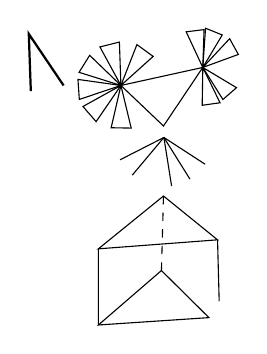
\begin{tikzpicture}[scale=.52]
\draw[thick] (-2.2,2.1)--(-2.25,3.5)--(-1.4,2.24);
\coordinate (u) at (0,2.24);\coordinate (v) at (2,2.68);
\draw (u)--(v)--(1.04,1.25)--(u);
\foreach \a in {42,92,136,172,209,257}{\draw (u)--++(\a:1.06)--++(\a+102:.49)--(u);}
\foreach \a in {47,86,115,-31,-64}{\draw (v)--++(\a:.96)--++(\a-108:.44)--(v);}
\foreach \a in {207,230,279,302,327}{\draw (1.05,.97)--++(\a:1.2);}
\draw (-.55,-1.75)--(1.04,-.46)--(2.36,-1.53)--cycle (-.55,-3.61)--(.99,-2.28)--(2.15,-3.43)--cycle
 (-.55,-3.61)--(-.55,-1.75) (2.36,-1.53)--(2.4,-3.03);
\draw[dashed] (1.04,-.46)--(.99,-2.28);
\end{tikzpicture}}

% L11–14 far right
$\unsure{\zeta_{1i}|\zeta_1\,i|\xi_1}\qquad i\in\{1,\ldots,6\}$

$1\ \underline{1}$

$(2\eta-\zeta)\mathbin{\unsure{\cdot|+}}\unsure{h_j|W_j|\xi_j}=2$

% L14–16 lower middle
\[
 \begin{aligned}
 &\mathfrak S_3\quad\sim\qquad 6^4=2^4\,3^4\quad\text{\textcircled{40}}\\
 &\begin{array}{r}81\\16\\\hline486\\81\phantom0\\\hline1296\end{array}
 \end{aligned}
\]

% L15–18 lower left
\[
 \begin{aligned}
 &\begin{matrix}F\\\downarrow\\E\end{matrix}
 \qquad\coprod_{i\in E}\ \prod_{j\in E-\{i\}}F_j\\
 &\unsure{\zeta'}\qquad \unsure{\zeta}= \eta-\deleted{\unsure{\zeta_j}}\zeta_k
 \end{aligned}
\]

% L18–21 lower centre left
\unsure{ou parties de|ou partitions|on particulier} \deleted{\unsure{telles que|telle que}} de \unsure{Card.|card.} 2 \unsure{jt} qui ne sont pas dans une fibre

% lower left edge
% margin note written sideways
\margin{$2\eta-\zeta\qquad 2\eta-\zeta_i-\zeta_j\qquad 4-2=2\qquad\zeta'_i-\zeta_i$}

% lower right edge
% margin note written sideways
\margin{$\dfrac{27\cdot16\cdot10}{6}=9\cdot16\cdot5=720=6!$}

% lower right L15–20
\figure{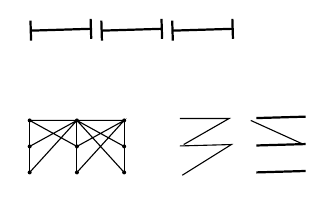
\begin{tikzpicture}[scale=.6]
\foreach \x in {0,1.5,3}{\draw[|-|,thick] (\x,3)--(\x+1.32,3.04);}
\foreach \x in {0,1,2}{\foreach \y in {0,.55,1.1}{\fill (\x,\y) circle (1.2pt);}\draw (\x,0)--(\x,1.1);}
\draw (0,1.1)--(2,1.1) (0,.55)--(1,1.1)--(2,0) (0,0)--(1,1.1)--(2,.55) (0,1.1)--(1,.55)--(2,1.1)--(1,0);
\foreach \y in {0,.57,1.15}{\draw[thick] (4.8,\y)--(5.84,\y+.03);}
\draw (3.18,.56)--(4.27,.59)--(3.23,-.06) (3.18,1.14)--(4.22,1.14)--(3.26,.59) (4.68,1.1)--(5.76,.61);
\end{tikzpicture}}

% bottom centre
\[
 \begin{aligned}&\deleted{\unsure{42}}\\&9\times9=81\\&3\times3\times3=27\\&54\end{aligned}
\]

% foot
\figure{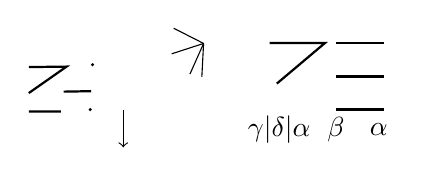
\begin{tikzpicture}[scale=.6]
\draw[thick] (0,.9)--(.8,.91)--(0,.35) (.74,.38)--(1.32,.39) (0,-.04)--(.68,-.04);
\fill (1.35,.95) circle (1pt); \fill (1.3,0) circle (1pt);
\draw[->] (2,0)--(2,-.8);
\foreach \y in {0,.7,1.41}{\draw[thick] (6.5,\y)--(7.52,\y);}
\draw[thick] (5.1,1.41)--(6.27,1.41)--(5.25,.55);
\node at (5.3,-.43) {$\unsure{\gamma|\delta|\alpha}$};\node at (6.5,-.43) {$\beta$};\node at (7.41,-.43) {$\alpha$};
\foreach \a in {153,198,246,267}{\draw (3.7,1.4)--++(\a:.71);}
\end{tikzpicture}}
% archive sheet number: 26
